\documentclass[12pt]{article}

\usepackage[utf8]{inputenc}
\usepackage{geometry}
\geometry{
    a4paper,
    total={170mm,257mm},
    left=25mm,
    right=25mm,
    top=25mm,
    bottom=25mm,
}
\usepackage{multicol}
\usepackage[font=small,labelfont=bf]{caption}
\setlength{\columnsep}{0.25cm}
\usepackage[inline]{enumitem}
\usepackage{bm}
\usepackage{amssymb}
\usepackage{xcolor}
\usepackage{mathtools} 
\setlength{\parindent}{0em}
\setlength{\parsep}{0em}
\usepackage{tikz}
\setlength{\parskip}{0em}
\usetikzlibrary{decorations.pathmorphing,patterns}
\usepackage[american,cuteinductors]{circuitikz}
\usetikzlibrary{shapes,arrows,circuits,calc,babel}
% Definition of blocks:
\tikzset{%
  block/.style    = {draw, thick, rectangle, minimum height = 3em,
    minimum width = 3em},
  sum/.style      = {draw, circle, node distance = 2cm}, % Adder
  input/.style    = {coordinate}, % Input
  output/.style   = {coordinate} % Output
}
% Defining string as labels of certain blocks.
\newcommand{\suma}{\Large$+$}
\newcommand{\inte}{$\displaystyle \int$}
\newcommand{\derv}{\huge$\frac{d}{dt}$}

\def\mf{\ensuremath\mathbf}
\def\mb{\ensuremath\mathbb}
\def\mc{\ensuremath\mathcal}
\def\lp{\ensuremath\left(}
\def\rp{\ensuremath\right)}
\def\lv{\ensuremath\left\lvert}
\def\rv{\ensuremath\right\rvert}
\def\lV{\ensuremath\left\lVert}
\def\rV{\ensuremath\right\rVert}
\def\lc{\ensuremath\left\{}
\def\rc{\ensuremath\right\}}
\def\ls{\ensuremath\left[}
\def\rs{\ensuremath\right]}
\def\bmx{\ensuremath\begin{bmatrix*}[r]}
\def\emx{\ensuremath\end{bmatrix*}}
\def\bmxc{\ensuremath\begin{bmatrix*}[c]}
\def\emxc{\ensuremath\end{bmatrix*}}
% \def\t{\lp t\rp}
% \def\k{\ls k\rs}

\newcommand{\demoex}[2]{\onslide<#1->\begin{color}{black!60} #2 \end{color}}
\newcommand{\demoexc}[3]{\onslide<#1->\begin{color}{#2} #3 \end{color}}
\newcommand{\anim}[3]{\onslide<#1->{\begin{color}{#2!60} #3 \end{color}}}
\newcommand{\ct}[1]{\lp #1\rp}
\newcommand{\dt}[1]{\ls #1\rs}

% \renewcommand{\familydefault}{\sfdefault}

\begin{document}
\begin{center}
\begin{large}
\textbf{Applied Linear Algebra in Data Analaysis}\\
\vspace{0.1cm}
\end{large}
\textbf{SVD \& Dimensionality Reduction Assignment}
\end{center}
\hrule
\vspace{1em}

\begin{large}
    \textbf{Marks: 14}
\end{large}

\begin{enumerate}
    \item For a square $\mf{A} \in\mb{R}^{n \times n}$, the SVD tells us how a unit sphere in $\mb{R}^n$ is distorted by the linear transformation performed by $\mf{A}$. This degree of distortion can be quantified using the singular values of $\mf{A}$, which is the 2-norm \textit{condition number},
    \[ \kappa = \frac{\sigma_1}{\sigma_n} \]
    \begin{enumerate}
        \item Explain why $\kappa \geq 1$? \textbf{[Marks: 1]}
        \item What is condition number of a singular matrix? \textbf{[Marks: 1]}
        \item If $\mf{A}$ is non-singular, show that $\kappa = \lV\mf{A}\rV_2\lV\mf{A}^{-1}\rV_2$ \textbf{[Marks: 1]}
        \item Condition numbers can also be defined based on other p-norms. The general p-norm condition number is given by, $\kappa_p = \lV\mf{A}\rV_p\lV\mf{A}^{-1}\rV_p$. Evaluate the 1-norm, 2-norm and $\infty$-norm condition numbers for the following matrices. How do these number compare with each other? \textbf{[Marks: 3]}
        \begin{enumerate*}[label={(\roman*)}]
            \item $\mf{A} = \bmx 1 & 0\\ 0 & 1\emx$;
            \item $\mf{A} = \bmx 1 & -1\\ 10 & -9\emx$;
            \item $\mf{A} = \bmx 1 & 5\\ -1 & 1\emx$.
        \end{enumerate*}
        \item Conditions numbers play an important role in practice. We had earlier an example of an ill-conditioned system $\mf{Ax} = \mf{b}$. Consider the following systems, where: \textbf{[Marks: 2]}
        \begin{enumerate*}[label={(\roman*)}] 
            \item $\mf{A}_1 = \bmx 1 & -1 \\ 10 & -9\emx$; and 
            \item $\mf{A}_2 = \bmx 1 & -10 \\ 1 & 10\emx$
         \end{enumerate*}.

        For $\mf{b} = \bmx 10 \\ 0\emx$, what are the solutions $\mf{x}_1\lp=\mf{A}_1^{-1}\mf{b}\rp$ and $\mf{x}_2\lp=\mf{A}_2^{-1}\mf{b}\rp$?  \textbf{[Marks: 2]}

        Suppose there is an error in the measurement of $\mf{b}$, and we have $\tilde{\mf{b}} = \bmx 9 \\ 1\emx$. The relative error in $\mf{b}$ is given by $\delta b = \frac{\lV \mf{b} - \tilde{\mf{b}}\rV_2}{\lV\mf{b}\rV_2}$. What are the new solutions $\tilde{\mf{x}}_1$ and $\tilde{\mf{x}}_2$? \textbf{[Marks: 2]}

        Calculate $\delta x_1$ and $\delta x_2$, the relative errors in $\mf{x}_1$ and $\mf{x}_2$, respectively? How do these compare to $\delta b$? \textbf{[Marks: 2]}

        \textit{Note: Through this problem, you should be able to see that an ill-conditioned system has a large condition number, which can amplify error and thus lead to large uncertainty in the solutions.}
    \end{enumerate}

    \item \textcolor{blue}{\textbf{[Programming]}} \textbf{Multilead Electrocardiogram}. A multi-lead electrocardiogram (ECG) refers to a cardiac monitoring technique that involves recording electrical activity from the heart using multiple electrodes placed on the body. Each lead provides a different perspective on the heart's electrical activity, allowing for a more comprehensive assessment of its function.

    In a standard 12-lead ECG, there are 10 electrodes placed on specific locations on the limbs and chest. These electrodes create 12 different ``views'' of the heart, each representing the electrical activity in a particular direction. The 12-lead ECG is widely used in clinical settings to diagnose various cardiac conditions, such as arrhythmias, ischemia, and other abnormalities.
    
    The source of the electrical potential measured as ECG through bipolar electrode is the 3D current dipole $\bm{\phi}\ct{t}$ formed by the electrical activtity of the cardiac muscle cells. 
    \[ \bm{\phi}\ct{t} = \bmx \phi_x\ct{t} & \phi_y\ct{t} & \phi_z\ct{t}\emx^\top \mb{R}^3 \]
    where, $\phi_x, \phi_y, \phi_z \in\mb{R}$ are the componets of the current dipole along the $x$, $y$, and $z$ axes. The voltage recorded by any bipolar lead $v\ct{t}$ is proportional to the component of the current dipole along a spatial direction $\mf{l} \in\mb{R}^3$.
    \[ v\ct{t} = \mf{l}^\top \bm{\phi}\ct{t} = \bm{\phi}\ct{t}^\top\mf{l} \]
    When the voltage is sampled at $N$ time instants separated by the sampling time $\Delta t$, the voltage recorded by the bipolar lead is given by the vector $\mf{v} \in\mb{R}^N$.
    \[ \mf{v} = \bm{\Phi} \mf{l} \]
    where, 
    \begin{itemize}
        \item $\mf{v} = \bmxc v\ct{0} & v\ct{\Delta t} & \cdots & v\ct{\ct{N-1}\Delta t} \emx^\top \in \mb{R}^N$
        \item $\bm{\Phi} =\bmx \bm{\phi}\ct{0} & \bm{\phi}\ct{\Delta t} & \cdots & \bm{\phi}\ct{\ct{N - 1}\Delta t} \emx^\top \in \mb{R}^{N \times 3}$
    \end{itemize}
    The 12 lead ECG measurement can now be represented as the following,
    \[ \mf{V} = \bm{\Phi} \mf{L} \]
    where, $\mf{V} \in \mb{R}^{N \times 12}$ is the matrix of the 12 lead ECG measurements, and $\mf{L} \in \mb{R}^{3 \times 12}$ is the matrix of the spatial directions of the 12 bipolar leads. 

    Assuming the 
    
    %The electrical activity of the heart recorded from the surface of the skin is the voltage $v\ct{t}$ recorded by a bipolar lead can be thought of a projection of a 3D vector $\mf{v}\ct{t}$ onto a 2D plane. The 3D vector $\mf{v}\ct{t}$ is the electrical potential at the heart at time $t$ and the 2D plane is the plane formed by the two electrodes of the bipolar lead. The 3D vector $\mf{v}\ct{t}$ can be decomposed into three orthogonal components, $\mf{v}\ct{t} = \mf{u}_1\ct{t} + \mf{u}_2\ct{t} + \mf{u}_3\ct{t}$, where $\mf{u}_1\ct{t}$, $\mf{u}_2\ct{t}$ and $\mf{u}_3\ct{t}$ are the three orthogonal components of the electrical potential at the heart at time $t$. The 2D projection of $\mf{v}\ct{t}$ onto the plane formed by the two electrodes of the bipolar lead is given by $\mf{v}\ct{t} = \mf{P}\mf{v}\ct{t}$, where $\mf{P}$ is a $2 \times 3$ matrix that projects the 3D vector $\mf{v}\ct{t}$ onto the 2D plane. The 2D voltage $v\ct{t}$ recorded by the bipolar lead is given by $v\ct{t} = \mf{c}^T\mf{v}\ct{t}$, where $\mf{c}$ is a $2 \times 1$ vector that represents the two electrodes of the bipolar lead.
    
    % electrical activity of the heart recorded from the surface of the skin is The voltage $v\ct{t}$ recorded by a bipolar lead can be thought of a projection of a 

    % \item Consider a system  $S$, which when probed with a test signal $x\lp  t\rp$, and the system responds with an output signal $y\lp t\rp$. The experiment is repeated $M$ times on the system by repeatedly applying the text signal to th system and the response of the system is sampled $y\ls n\rs$ and recorded for a for a fixed duration of time $0 \leq n \leq N$. An example of the response of the system for the different experiments are shown below ($N = 100$),\vspace{-0.25cm}
    % \begin{center}
    % 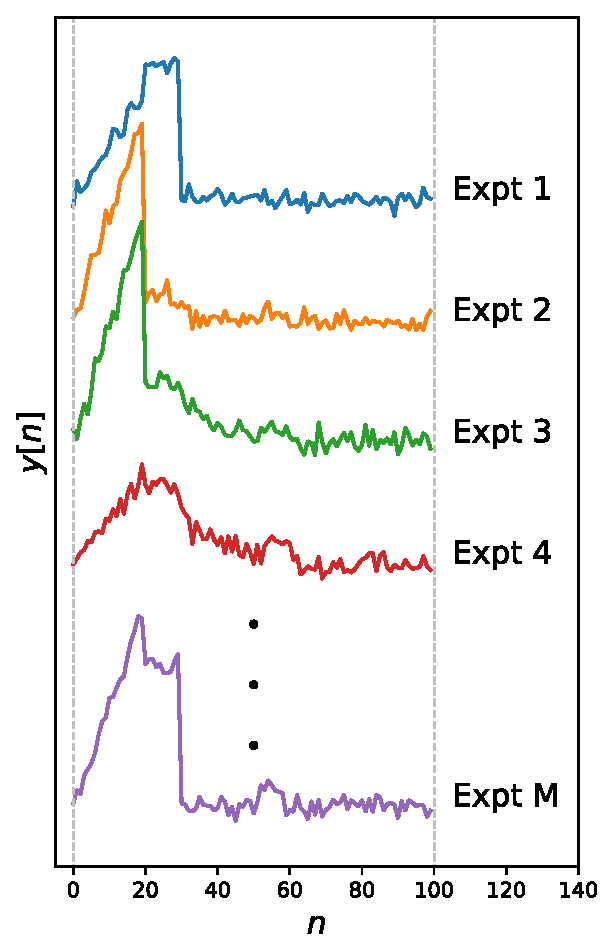
\includegraphics[width=0.7\columnwidth]{sections/figs/trig_expt.eps}
    % \end{center}\vspace{-0.3cm}
    % We know from the physics of the system that the system response to the test signal for the $j^{th}$ experiment given is given by ,
    % \[ y_j\ls n \rs = \sum_{i=1}^{K} w_{ji}\phi_i\ls n\rs + \nu_j\ls n\rs\]
    % where, $n$ is time index; $N$ is the number of data points recorded on each experiment; $\phi_i\ls n\rs, 1 \leq i \leq K$ are characteristic signals of the system; $w_{ji}$ are the weights that determine the amount of the $\phi_i$ present in the output $y_j$ for the $j^{th}$ experiment; and $\nu_j\ls n\rs$ is measurement noise present in the $j^{th}$ experiments. Additionally, we also know that
    % $$ \phi_i^T\phi_j = \sum_{l=0}^{N-1} \phi_i\ls l \rs\phi_j\ls l\rs = \begin{cases} 0 & i \neq j \\ 1 & i = j \end{cases} $$

    % Data from one such experiment is provided in the CSV file (trigexpt.csv) which contains an array of data where the rows correspond to system response for the different experiments, and the columns correspond to  different time index. Using this data identify the different characteristic signals $\phi_i$ for the system, along with the weights $w_{ji}$ for the different experiments. You must also ensure that the data is explained with least number characteristic signal, i.e. $K$ should be as low as possible. Explain how you chose $K$.l
\end{enumerate}

\end{document}